%%
%% Template feito com base no AbnTex2 para o curso de Estatística da UFG
%% Further information about abnTeX2 are available on https://github.com/abntex/abntex2
%%https://www.abntex.net.br/
%%

%%%%%%%%%%%%%%%%%%%%%%%%%%%%%%%%%%%%%%%%%%%%%%%%%%%%%%%%%%%%%%%%%%%%%%%%%%%%%%%%%%%%%%%%%%
%% Modelo de TCC para as seguintes matrizes:
%% - Matriz de 2009, aprovada em ....
%% - Matriz de 2019, aprovada em ....
%%
%% Data da última atualização: 18 de dezembro de 2025.
%%%%%%%%%%%%%%%%%%%%%%%%%%%%%%%%%%%%%%%%%%%%%%%%%%%%%%%%%%%%%%%%%%%%%%%%%%%%%%%%%%%%%%%%%%%


%%%%%%%%%%%%%%%%%%%%%%%%%%% OBSERVAÇÃO %%%%%%%%%%%%%%%%%%%%%%%%%%%%%%%%%%%%%%%%%%%%%%%%%%%%
%% Este modelo foi formulado pelo NDE-Estatística-IME/UFG
%% É de responsabilidade do(a) discente o cumprimento das Normas de TCC, bem como as normas da ABNT
%% e, portanto, fazer as alterações, se necessárias, para adaptação às normas da ABNT vigente.
%%%%%%%%%%%%%%%%%%%%%%%%%%%%%%%%%%%%%%%%%%%%%%%%%%%%%%%%%%%%%%%%%%%%%%%%%%%%%%%%%%%%%%%%%%%


\documentclass[
	% -- opções da classe memoir --
	12pt,				% tamanho da fonte
	openright,			% capítulos começam em pág ímpar (insere página vazia caso preciso)
	oneside,			% para impressão em recto e verso. Oposto a oneside
	a4paper,			% tamanho do papel.
	sumario = tradicional,
	% -- opções da classe abntex2 --
	%chapter=TITLE,		% títulos de capítulos convertidos em letras maiúsculas
	%section=TITLE,		% títulos de seções convertidos em letras maiúsculas
	%subsection=TITLE,	% títulos de subseções convertidos em letras maiúsculas
	%subsubsection=TITLE,% títulos de subsubseções convertidos em letras maiúsculas
	% -- opções do pacote babel --
	english,			% idioma adicional para hifenização
         %portugues,          % o último idioma é o principal do documento
	brazil,				% o último idioma é o principal do documento
    %%%%%%%%%%%%
        %eek: colocação da opção para o sumario ter formatação tradicional
        %sumario=tradicional             % título no formato tradicional
	]{abntex2}

% ---
% Pacotes básicos
% --
\usepackage{times} %{lmodern}	% Usa a fonte Latin Modern
\usepackage[T1]{fontenc}% Selecao de codigos de fonte.
\usepackage[utf8]{inputenc}% Codificacao do documento (conversão automática dos acentos)
\usepackage{indentfirst}	% Indenta o primeiro parágrafo de cada seção.
\usepackage{color}		% Controle das cores
\usepackage{graphicx}	% Inclusão de gráficos
\graphicspath{ {./figuras/} }
\usepackage{microtype} 	% para melhorias de justificação
\usepackage{array} %permite o uso de tabelas
\usepackage{longtable} %permite o uso de tabelas personalizadas
\usepackage{rotating} %permite rotacionar imagens
%\usepackage{tikz} %permite o desenho de formas geométricas simples dadas suas características
\usepackage{TCC_EST_IME} %% Customização da classe abnTeX2 para o TCC da Estatística do IME-UFG
\usepackage{ragged2e}
\usepackage{csquotes}
\usepackage{amsfonts}
\usepackage{amsmath}
\usepackage{amssymb}
\usepackage{graphicx, epsfig}
\usepackage{indentfirst}
\usepackage{setspace}
\usepackage{lscape}
\usepackage{multirow}
\usepackage{float} %% incompatível com quadros
\usepackage{listings}
\usepackage{comment}
\usepackage{booktabs}
\usepackage{bm, color}
\usepackage{hyperref}
\usepackage{tikz}
\usepackage{xypic}
\usepackage{url}
\usepackage{icomma} %retirar o espaço que o latex coloca automaticamente após vírgulas
\usepackage{pdfpages} %incluir páginas de pdf






%%----------- Pacotes adicionais (do autor):
%% Adicionar aqui os pacotes adicionais usados

%\usepackage{}

%%----------------------------------------------





%%% OUTRAS CONFIGURAÇÕES:

%%-------------------------------------------------------
% Pacotes de citações
% ---
\usepackage[brazilian,hyperpageref]{backref}	 % Paginas com as citações na bibl
%\usepackage[alf]{abntex2cite}	% Citações padrão ABNT
\usepackage[alf,
abnt-emphasize = bf, % destaca o titulo da revista ou livro em negrito;
abnt-etal-list = 3, % trabalhos com mais de 3 autores recebem et al.,;
abnt-etal-text = it, % escreve o et al., em italico;
abnt-and-type = e, % usa o carater '&' no lugar de 'e' para mais de um autor;
abnt-last-names = abnt, % trata sobrenomes 'estritamente' conforme a ABNT; e
abnt-repeated-author-omit = no % autores com + de uma entrada recebem '____.'
]{abntex2cite}
% ---
% CONFIGURAÇÕES DE PACOTES
% ---
% Configurações do pacote backref
% Usado sem a opção hyperpageref de backref
\renewcommand{\backrefpagesname}{Citado na(s) página(s):~}
% Texto padrão antes do número das páginas
\renewcommand{\backref}{}
% Define os textos da citação
\renewcommand*{\backrefalt}[4]{
	\ifcase #1 %
		Nenhuma citação no texto.%
	\or
		Citado na página #2.%
	\else
		Citado #1 vezes nas páginas #2.%
	\fi}%
%%-------------------------------------------------------



%%-------------------------------------------------------
% ---
% Configurações de aparência do PDF final

% alterando o aspecto da cor azul
\definecolor{blue}{RGB}{41,5,195}

% informações do PDF
\makeatletter
\hypersetup{
     	%pagebackref=true,
		pdftitle={\@title},
		pdfauthor={\@author},
    	pdfsubject={\imprimirpreambulo},
	    pdfcreator={\@author},
		pdfkeywords={palavra-chave}{palavra-chave}{palavra-chave},
		colorlinks=true,       		% false: boxed links; true: colored links
    	linkcolor=black,          	% color of internal links
    	citecolor=black,        		% color of links to bibliography
    	filecolor=magenta,      		% color of file links
		urlcolor=black,
		bookmarksdepth=4}
\makeatother
% ---

% ---
% Posiciona figuras e tabelas no topo da página quando adicionadas sozinhas
% em um página em branco. Ver https://github.com/abntex/abntex2/issues/170
\makeatletter
\setlength{\@fptop}{5pt} % Set distance from top of page to first float
\makeatother
% ---

% % ---
% % Possibilita criação de Quadros e Lista de quadros.
% % Ver https://github.com/abntex/abntex2/issues/176
% %
% \newcommand{\quadroname}{Quadro}
% \newcommand{\listofquadrosname}{Lista de quadros}
% \newfloat[chapter]{quadro}{loq}{\quadroname}
% \newlistof{listofquadros}{loq}{\listofquadrosname}
% \newlistentry{quadro}{loq}{0}

% % configurações para atender às regras da ABNT
% \setfloatadjustment{quadro}{\centering}
% \counterwithout{quadro}{chapter}
% \renewcommand{\cftquadroname}{\quadroname\space}
% \renewcommand*{\cftquadroaftersnum}{\hfill--\hfill}

% \setfloatlocations{quadro}{hbtp} % Ver https://github.com/abntex/abntex2/issues/176
% % ---


% ---
% Possibilita criação de Lista de símbolos.
% Ver https://github.com/abntex/abntex2/issues/104
%
\makeatletter
\newcommand\criarsimbolo[2]{%
  \write\@auxout{\noexpand\@writefile{sbl}{\noexpand\item[#1] #2}}}
\newcommand\imprimirlistadesimbolos{%
  \begin{simbolos}
   \@starttoc{sbl}
  \end{simbolos}}
\makeatother

% ---
% Possibilita criação de Lista de siglas e abreviaturas.
%
\makeatletter
\newcommand\criarsigla[2]{%
  \write\@auxout{\noexpand\@writefile{sbs}{\noexpand\item[#1] #2}}}
\newcommand\imprimirlistadesiglas{%
  \begin{siglas}
   \@starttoc{sbs}
  \end{siglas}}
\makeatother


% ---
% Espaçamentos entre linhas e parágrafos
% ---

% O tamanho do parágrafo é dado por:
\setlength{\parindent}{1.25cm}

% Controle do espaçamento entre um parágrafo e outro:
\setlength{\parskip}{0.2cm}  % tente também \onelineskip

%Espaçamento padrão:
\OnehalfSpacing


% ----------------------------------------------------------
% Informações de Lista de Figuras
% ----------------------------------------------------------

%\addto\captionsbrazil{\renewcommand{\listfigurename}{Lista de figuras}}

% ----------------------------------------------------------
% Informações de dados para CAPA e FOLHA DE ROSTO
% ----------------------------------------------------------
\titulo{Título do trabalho em letras minúsculas e sem ponto final: subtítulo se houver}
\autor{Nome do(a) autor(a)}
\local{Goiânia}
\data{Ano}
\orientador{Nome do(a) orientador(a)}
%\coorientador{Nome do(a) coorientador(a)}  %% se houver
\instituicao{%
  Universidade Federal de Goiás
  \par
  Instituto de Matemática e Estatística
  \par
  Bacharelado em Estatística}
\tipotrabalho{Trabalho de Conclusão de Curso (TCC)}

%% matriz 2019
\preambulo{Trabalho de
      Conclusão de Curso apresentado ao
      Curso de  Bacharelado em Estatística da
      Universidade Federal de Goiás para aprovação no componente curricular
      TCC, como parte das exigências para a obtenção do título de bacharel em Estatística.\linebreak
\textbf{Orientador}: \imprimirorientador
%\linebreak \textbf{Coorientador}: \imprimircoorientador  %% ser houver
}

% ----------------------------------------------------------
% Compila o índice
% ---
\makeindex
% ----------------------------------------------------------



% ----------------------------------------------------------
% Início do documento
% ----------------------------------------------------------
\begin{document}
\selectlanguage{brazil}

% Retira espaço extra obsoleto entre as frases.
\frenchspacing
%espaçamento

% ----------------------------------------------------------
% ----------------------------------------------------------
% ELEMENTOS PRÉ-TEXTUAIS
%---
\pretextual
% ----------------------------------------------------------

% ----------------------------------------------------------
% Capa (obrigatória)
%---
\imprimircapa
% ----------------------------------------------------------
%Inserir TECA - Termo de Ciência e de Autorização
%---
%\includepdf[pages=-, scale=0.9]{TECA_assinado_FernandoNery.pdf}
{
\centerline{Incluir aqui o TECA (arquivo pdf) gerada do processo SEI referente ao TCC.\\}
%\includepdf[pages=-, scale=0.9]{SEI_5831481_Termo_de_Ciencia_e_de_Autorizacao_TCCG__RI__TECA.pdf}
\centerline{Acima estão comentados os comandos para tal inclusão.\\ }

\centerline{(Lembre-se de comentar este texto e deixar apenas o arquivo pdf.)}
}
% ----------------------------------------------------------

% Folha de rosto (obrigatória)
% (o * indica que haverá a ficha bibliográfica)
%---
\imprimirfolhaderosto
% ----------------------------------------------------------
% ----------------------------------------------------------
% Inserir a ficha bibliografica
%---

\centerline{Incluir aqui a ficha catalográfica (arquivo pdf) gerada pelo aplicativo da Biblioteca.\\}
%\includepdf[scale=0.9]{ficha_catalografica.pdf}
\centerline{Acima estão comentados os comandos para tal inclusão.\\ }

\centerline{(Lembre-se de comentar este texto e deixar apenas o arquivo pdf.)}
\newpage

% ----------------------------------------------------------% ----------------------------------------------------------



% ----------------------------------------------------------
%Inserir errata (caso houver)
%---
%\input{capitulos/prett_errata.tex}
% ----------------------------------------------------------



% ----------------------------------------------------------
% Inserir folha de aprovação (obrigatória)
%---
%\includepdf[pages=-, scale=0.9]{certidaoAprovacao.pdf}
{
\centerline{Incluir aqui a ata de defesa (arquivo pdf) gerada do processo SEI referente ao TCC.\\}
%\includepdf[pages=-, scale=0.9]{SEI_5808281_Ata_de_Defesa_de_Trabalho_de_Conclusao_de_Curso.pdf}
\centerline{Acima estão comentados os comandos para tal inclusão.\\ }

\centerline{(Lembre-se de comentar este texto e deixar apenas o arquivo pdf.)}
\newpage
}
% ----------------------------------------------------------
% Dedicatória/Agradecimentos/Epígrafe (opcionais)
%---

% ---
% Dedicatória (opcional)
% ---
\begin{dedicatoria}
   \vspace*{\fill}
   \vspace*{\fill}
   \vspace*{\fill}
   \vspace*{\fill}
   \flushright
   \noindent
   \textit{À alguém...}
   \vspace*{48pt}
\end{dedicatoria}
% ---

% ---
% Agradecimentos (opcional)
% ---
\begin{agradecimentos}
Liste a quem deseja agradecer (opcional) em ordem decrescente de importância, evitando um número muito extenso de pessoas.
Os agradecimentos parágrafo parágrafo parágrafo parágrafo parágrafo parágrafo parágrafo parágrafo parágrafo parágrafo parágrafo parágrafo parágrafo parágrafo parágrafo parágrafo parágrafo parágrafo parágrafo parágrafo parágrafo parágrafo parágrafo parágrafo parágrafo parágrafo parágrafo parágrafo parágrafo parágrafo parágrafo parágrafo parágrafo parágrafo parágrafo parágrafo parágrafo parágrafo parágrafo parágrafo parágrafo 

parágrafo parágrafo parágrafo parágrafo parágrafo parágrafo parágrafo parágrafo parágrafo parágrafo parágrafo parágrafo parágrafo parágrafo parágrafo parágrafo parágrafo parágrafo parágrafo parágrafo parágrafo parágrafo parágrafo parágrafo parágrafo parágrafo parágrafo parágrafo parágrafo parágrafo parágrafo parágrafo parágrafo parágrafo parágrafo parágrafo parágrafo parágrafo parágrafo parágrafo parágrafo parágrafo parágrafo parágrafo parágrafo parágrafo parágrafo parágrafo parágrafo parágrafo parágrafo parágrafo parágrafo parágrafo parágrafo 

\end{agradecimentos}
% ---

% ---
% Epígrafe (opcional)
% ---
\begin{epigrafe}
    \vspace*{\fill}
	\begin{flushright}
		''Elemento opcional, que traz a citação de um pensamento seguido de autoria e que represente a gênese da obra (seu trabalho). Não há necessidade de escrever o título “Epígrafe”. Usar letras minúsculas alinhadas à direita da parte inferior da folha'' (Alguém, Livro, ano)
        \vspace*{48pt}
	\end{flushright}
\end{epigrafe}
% ----------------------------------------------------------


% ----------------------------------------------------------
% Resumos (obrigatórios)
%---

% resumo em português
\setlength{\absparsep}{18pt} % ajusta o espaçamento dos parágrafos do resumo
\begin{resumo}
 Parágrafo Parágrafo Parágrafo Parágrafo Parágrafo Parágrafo Parágrafo Parágrafo Parágrafo Parágrafo Parágrafo Parágrafo Parágrafo Parágrafo Parágrafo Parágrafo Parágrafo Parágrafo Parágrafo Parágrafo Parágrafo Parágrafo Parágrafo Parágrafo Parágrafo Parágrafo Parágrafo Parágrafo Parágrafo Parágrafo Parágrafo Parágrafo Parágrafo Parágrafo Parágrafo Parágrafo Parágrafo Parágrafo Parágrafo Parágrafo Parágrafo Parágrafo Parágrafo Parágrafo Parágrafo Parágrafo Parágrafo Parágrafo Parágrafo Parágrafo Parágrafo Parágrafo Parágrafo Parágrafo Parágrafo .

{Palavras-chave}: Palavra-chave. Palavra-chave. Palavra-chave.
\end{resumo}

% resumo em inglês
\begin{resumo}[Abstract]
 \begin{otherlanguage*}{english}
   This is the english abstract.

   \vspace{\onelineskip}
 
   \noindent 
{Keywords}: Keyword. Keyword. Keyword.
 \end{otherlanguage*}
\end{resumo}



% ----------------------------------------------------------


% ----------------------------------------------------------
% Listas (opcionais)
%---
%\input{capitulos/prett_listas.tex}
% ----------------------------------------------------------


% ----------------------------------------------------------
% Inserir o Sumário (obrigatório)
%---
\pdfbookmark[0]{\contentsname}{toc}
\tableofcontents*
\cleardoublepage
% ----------------------------------------------------------




% ----------------------------------------------------------
% ----------------------------------------------------------
% ELEMENTOS TEXTUAIS
%---
\textual
\setcounter{chapter}{1}
\counterwithout{equation}{chapter}
% ----------------------------------------------------------

%-----------------------------------------------------
%% Os títulos do modelo são sugestões, podendo ser alterados.
%% Introdução e Conclusão são obrigatórios.
%-----------------------------------------------------

% ---
% Introdução (sem numeração, mas presente no Sumário)
% ---
\chapter*[Introdução]{Introdução}\label{cap_introducao}
\addcontentsline{toc}{chapter}{Introdução}
% ---


Segundo a norma de formatação dos trabalhos de final de curso de Estatística da Universidade Federal de Goiás (IME/UFG), toda abreviatura deve ser definida antes de utilizada.\criarsigla{IME}{Instituto de Matemática e Estatística}\criarsigla{UFG}{Universidade Federal de Goiás}

Outro exemplo. Os dados foram obtidos no site do Instituto Brasileiro de Geografia e Estatística (IBGE). \criarsigla{IBGE}{Instituto Brasileiro de Geografia e Estatística}

Do mesmo modo, é imprescindível definir os símbolos, tal como o conjunto dos números reais $\mathbb{R}$ e o conjunto vazio $\emptyset$.
\criarsimbolo{$\mathbb{R}$}{Conjunto dos números reais} \criarsimbolo{$\emptyset$}{Conjunto vazio}

Parágrafo Parágrafo Parágrafo Parágrafo Parágrafo Parágrafo Parágrafo Parágrafo Parágrafo Parágrafo Parágrafo Parágrafo Parágrafo Parágrafo Parágrafo Parágrafo Parágrafo Parágrafo Parágrafo Parágrafo Parágrafo Parágrafo Parágrafo Parágrafo Parágrafo Parágrafo Parágrafo Parágrafo Parágrafo Parágrafo 

Parágrafo Parágrafo Parágrafo Parágrafo Parágrafo Parágrafo Parágrafo Parágrafo Parágrafo Parágrafo Parágrafo Parágrafo Parágrafo Parágrafo Parágrafo Parágrafo Parágrafo Parágrafo Parágrafo Parágrafo Parágrafo Parágrafo Parágrafo Parágrafo 

Parágrafo Parágrafo Parágrafo Parágrafo Parágrafo Parágrafo Parágrafo Parágrafo Parágrafo Parágrafo Parágrafo Parágrafo Parágrafo Parágrafo Parágrafo Parágrafo Parágrafo Parágrafo Parágrafo Parágrafo Parágrafo Parágrafo Parágrafo Parágrafo Parágrafo Parágrafo Parágrafo Parágrafo 

Parágrafo Parágrafo Parágrafo Parágrafo Parágrafo Parágrafo Parágrafo Parágrafo Parágrafo Parágrafo Parágrafo Parágrafo Parágrafo Parágrafo Parágrafo Parágrafo Parágrafo Parágrafo Parágrafo Parágrafo Parágrafo Parágrafo Parágrafo Parágrafo Parágrafo Parágrafo Parágrafo Parágrafo Parágrafo Parágrafo 

Parágrafo Parágrafo Parágrafo Parágrafo Parágrafo Parágrafo Parágrafo Parágrafo Parágrafo Parágrafo Parágrafo Parágrafo Parágrafo Parágrafo Parágrafo Parágrafo Parágrafo Parágrafo Parágrafo Parágrafo Parágrafo Parágrafo Parágrafo Parágrafo 

Parágrafo Parágrafo Parágrafo Parágrafo Parágrafo Parágrafo Parágrafo Parágrafo Parágrafo Parágrafo Parágrafo Parágrafo Parágrafo Parágrafo Parágrafo Parágrafo Parágrafo Parágrafo Parágrafo Parágrafo Parágrafo Parágrafo Parágrafo Parágrafo Parágrafo Parágrafo Parágrafo Parágrafo

Parágrafo Parágrafo Parágrafo Parágrafo Parágrafo Parágrafo Parágrafo Parágrafo Parágrafo Parágrafo Parágrafo Parágrafo Parágrafo Parágrafo Parágrafo Parágrafo Parágrafo Parágrafo Parágrafo Parágrafo Parágrafo Parágrafo Parágrafo Parágrafo Parágrafo Parágrafo Parágrafo Parágrafo Parágrafo Parágrafo 

Parágrafo Parágrafo Parágrafo Parágrafo Parágrafo Parágrafo Parágrafo Parágrafo Parágrafo Parágrafo Parágrafo Parágrafo Parágrafo Parágrafo Parágrafo Parágrafo Parágrafo Parágrafo Parágrafo Parágrafo Parágrafo Parágrafo Parágrafo Parágrafo 

Parágrafo Parágrafo Parágrafo Parágrafo Parágrafo Parágrafo Parágrafo Parágrafo Parágrafo Parágrafo Parágrafo Parágrafo Parágrafo Parágrafo Parágrafo Parágrafo Parágrafo Parágrafo Parágrafo Parágrafo Parágrafo Parágrafo Parágrafo Parágrafo Parágrafo Parágrafo Parágrafo Parágrafo


%-----------------------------------------------------

% ---
% Capitulo de revisão de literatura
% ---

\chapter{Revisão Bibliográfica}\label{cap_rev_bibliografica}

Aqui deve ser feita uma revisão preliminar da literatura. Texto da Revisão Bibliográfica Parágrafo Parágrafo Parágrafo Parágrafo Parágrafo Parágrafo Parágrafo Parágrafo Parágrafo Parágrafo Parágrafo Parágrafo Parágrafo Parágrafo Parágrafo Parágrafo Parágrafo Parágrafo Parágrafo Parágrafo Parágrafo Parágrafo Parágrafo Parágrafo Parágrafo Parágrafo Parágrafo Parágrafo 

\section{Título da Seção 1}


Citações de bibliográficas podem ser feitas de forma corrente no texto, utilizando \citeonline{araujoclasse}. Podem ser citadas entre parênteses, quando a referência não fizer parte do texto \cite{morettin2017estatistica}.

Citações com 2 autores ficam da seguinte forma:
\citeonline{colosimo2006analise} ou \cite{colosimo2006analise}.

Citações com 3 ou mais autores ficam da seguinte forma:  \citeonline{carvalho2011analise} ou \cite{carvalho2011analise}.

Citações de páginas da internet devem ser feitas por \citeonline{FigCurvaAngulos} ou \cite{FigCurvaAngulos}.

O software \citeonline{citacaoR} deve ser citado na seção de resultados.

\section{Título da Seção 2}

Parágrafo Parágrafo Parágrafo Parágrafo Parágrafo Parágrafo Parágrafo Parágrafo Parágrafo Parágrafo Parágrafo Parágrafo Parágrafo Parágrafo Parágrafo Parágrafo Parágrafo Parágrafo Parágrafo Parágrafo Parágrafo Parágrafo Parágrafo Parágrafo Parágrafo Parágrafo Parágrafo Parágrafo Parágrafo Parágrafo 

Parágrafo Parágrafo Parágrafo Parágrafo Parágrafo Parágrafo Parágrafo Parágrafo Parágrafo Parágrafo Parágrafo Parágrafo Parágrafo Parágrafo Parágrafo Parágrafo Parágrafo Parágrafo Parágrafo Parágrafo Parágrafo Parágrafo Parágrafo Parágrafo 

Parágrafo Parágrafo Parágrafo Parágrafo Parágrafo Parágrafo Parágrafo Parágrafo Parágrafo Parágrafo Parágrafo Parágrafo Parágrafo Parágrafo Parágrafo Parágrafo Parágrafo Parágrafo Parágrafo Parágrafo Parágrafo Parágrafo Parágrafo Parágrafo Parágrafo Parágrafo Parágrafo Parágrafo 

\subsection{Título da Subseção}

Parágrafo Parágrafo Parágrafo Parágrafo Parágrafo Parágrafo Parágrafo Parágrafo Parágrafo Parágrafo Parágrafo Parágrafo Parágrafo Parágrafo Parágrafo Parágrafo Parágrafo Parágrafo Parágrafo Parágrafo Parágrafo Parágrafo Parágrafo Parágrafo Parágrafo Parágrafo Parágrafo Parágrafo Parágrafo Parágrafo 

Parágrafo Parágrafo Parágrafo Parágrafo Parágrafo Parágrafo Parágrafo Parágrafo Parágrafo Parágrafo Parágrafo Parágrafo Parágrafo Parágrafo Parágrafo Parágrafo Parágrafo Parágrafo Parágrafo Parágrafo Parágrafo Parágrafo Parágrafo Parágrafo 

Parágrafo Parágrafo Parágrafo Parágrafo Parágrafo Parágrafo Parágrafo Parágrafo Parágrafo Parágrafo Parágrafo Parágrafo Parágrafo Parágrafo Parágrafo Parágrafo Parágrafo Parágrafo Parágrafo Parágrafo Parágrafo Parágrafo Parágrafo Parágrafo Parágrafo Parágrafo Parágrafo Parágrafo 
%-----------------------------------------------------

% ---
% Capitulo da Metodologia
% ---

\chapter{Metodologia}\label{cap_metodologia}

Texto da Metodologia Parágrafo Parágrafo Parágrafo Parágrafo Parágrafo Parágrafo Parágrafo Parágrafo Parágrafo Parágrafo Parágrafo Parágrafo Parágrafo Parágrafo Parágrafo Parágrafo Parágrafo Parágrafo Parágrafo Parágrafo Parágrafo Parágrafo Parágrafo Parágrafo Parágrafo Parágrafo Parágrafo Parágrafo Parágrafo Parágrafo 

\section{Título da Seção 1}

Detalhamento da metodologia a ser utilizada: caracterização da pesquisa, população, amostra, instrumentos de medida. 


Este parágrafo apresenta como referenciar a figura no texto, requisito obrigatório da ABNT.  Primeira opção, utilizando \texttt{autoref}: Ver a \autoref{fig1}. Segunda opção, utilizando  \texttt{ref}: Ver a Figura \ref{fig1}.

\begin{figure}[h] 
\centering 
\caption{Exemplo de gráfico}\label{fig1} 
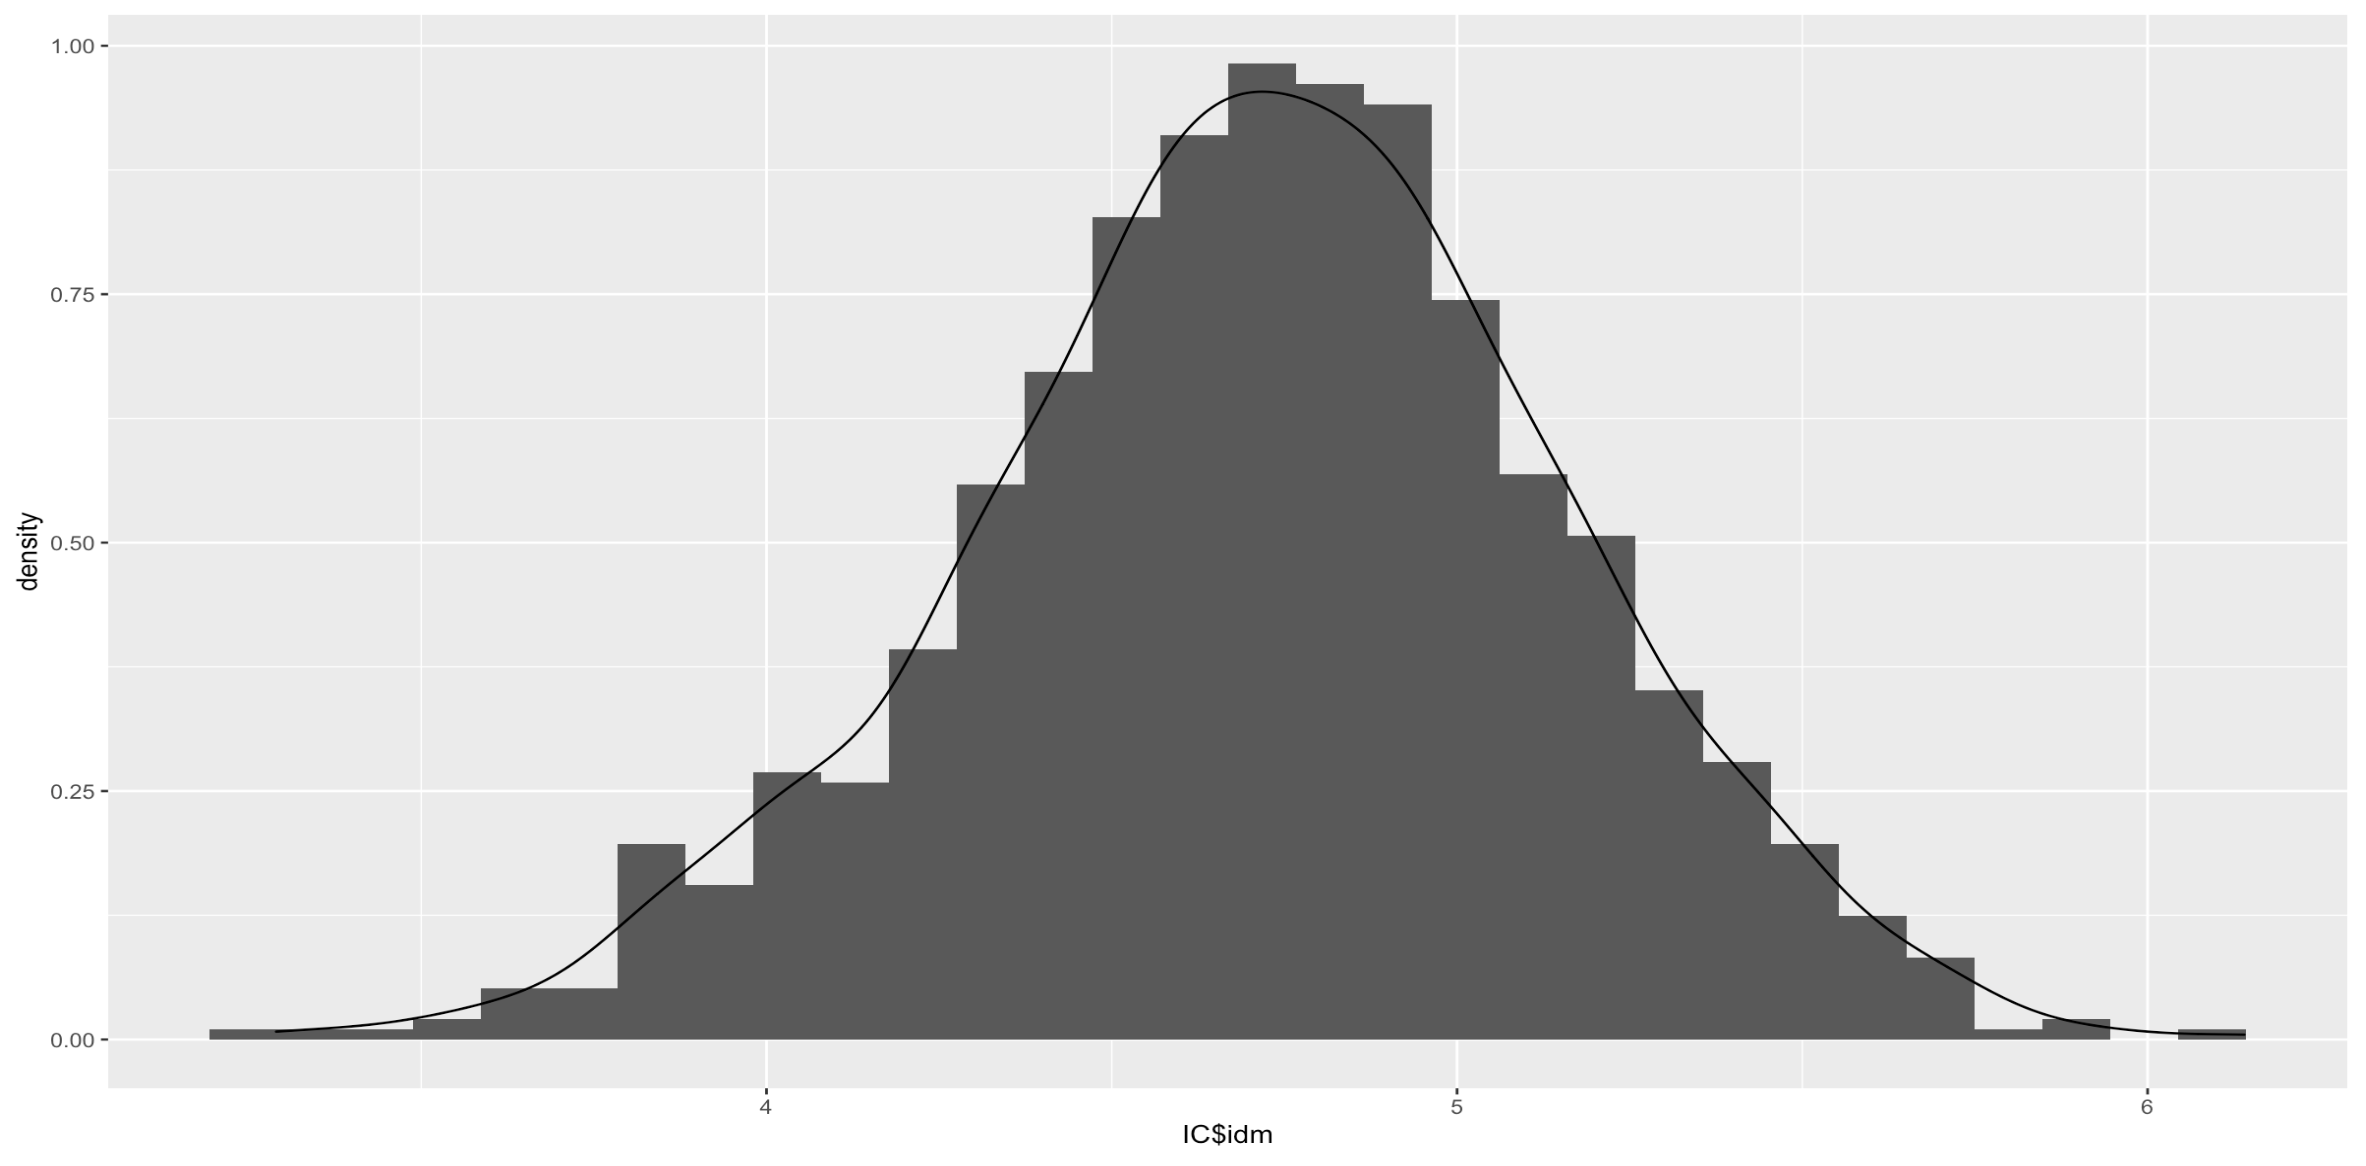
\includegraphics[scale=0.30]{figuras/hist.png}
\fonte{Elaborado pelo autor}
\end{figure}


Parágrafo Parágrafo Parágrafo Parágrafo Parágrafo Parágrafo Parágrafo Parágrafo Parágrafo Parágrafo Parágrafo Parágrafo Parágrafo Parágrafo Parágrafo Parágrafo Parágrafo Parágrafo Parágrafo Parágrafo Parágrafo Parágrafo Parágrafo Parágrafo Parágrafo Parágrafo Parágrafo Parágrafo Parágrafo Parágrafo 

Parágrafo Parágrafo Parágrafo Parágrafo Parágrafo Parágrafo Parágrafo Parágrafo Parágrafo Parágrafo Parágrafo Parágrafo Parágrafo Parágrafo Parágrafo Parágrafo Parágrafo Parágrafo Parágrafo Parágrafo Parágrafo Parágrafo Parágrafo Parágrafo 

Parágrafo Parágrafo Parágrafo Parágrafo Parágrafo Parágrafo Parágrafo Parágrafo Parágrafo Parágrafo Parágrafo Parágrafo Parágrafo Parágrafo Parágrafo Parágrafo Parágrafo Parágrafo Parágrafo Parágrafo Parágrafo Parágrafo Parágrafo Parágrafo Parágrafo Parágrafo Parágrafo Parágrafo 

\section{Título da Seção 2}

Parágrafo Parágrafo Parágrafo Parágrafo Parágrafo Parágrafo Parágrafo Parágrafo Parágrafo Parágrafo Parágrafo Parágrafo Parágrafo Parágrafo Parágrafo Parágrafo Parágrafo Parágrafo Parágrafo Parágrafo Parágrafo Parágrafo Parágrafo Parágrafo Parágrafo Parágrafo Parágrafo Parágrafo Parágrafo Parágrafo 

Parágrafo Parágrafo Parágrafo Parágrafo Parágrafo Parágrafo Parágrafo Parágrafo Parágrafo Parágrafo Parágrafo Parágrafo Parágrafo Parágrafo Parágrafo Parágrafo Parágrafo Parágrafo Parágrafo Parágrafo Parágrafo Parágrafo Parágrafo Parágrafo 

Parágrafo Parágrafo Parágrafo Parágrafo Parágrafo Parágrafo Parágrafo Parágrafo Parágrafo Parágrafo Parágrafo Parágrafo Parágrafo Parágrafo Parágrafo Parágrafo Parágrafo Parágrafo Parágrafo Parágrafo Parágrafo Parágrafo Parágrafo Parágrafo Parágrafo Parágrafo Parágrafo Parágrafo

\subsection{Título da Subseção}

Parágrafo Parágrafo Parágrafo Parágrafo Parágrafo Parágrafo Parágrafo Parágrafo Parágrafo Parágrafo Parágrafo Parágrafo Parágrafo Parágrafo Parágrafo Parágrafo Parágrafo Parágrafo Parágrafo Parágrafo Parágrafo Parágrafo Parágrafo Parágrafo Parágrafo Parágrafo Parágrafo Parágrafo Parágrafo Parágrafo 

Parágrafo Parágrafo Parágrafo Parágrafo Parágrafo Parágrafo Parágrafo Parágrafo Parágrafo Parágrafo Parágrafo Parágrafo Parágrafo Parágrafo Parágrafo Parágrafo Parágrafo Parágrafo Parágrafo Parágrafo Parágrafo Parágrafo Parágrafo Parágrafo 

Parágrafo Parágrafo Parágrafo Parágrafo Parágrafo Parágrafo Parágrafo Parágrafo Parágrafo Parágrafo Parágrafo Parágrafo Parágrafo Parágrafo Parágrafo Parágrafo Parágrafo Parágrafo Parágrafo Parágrafo Parágrafo Parágrafo Parágrafo Parágrafo Parágrafo Parágrafo Parágrafo Parágrafo

%-----------------------------------------------------

% ---
% Capitulo de Resultados
% ---

\chapter{Resultados}\label{cap_resultados}

Introdução do Parágrafo de Resultados Parágrafo Parágrafo Parágrafo Parágrafo Parágrafo Parágrafo Parágrafo Parágrafo Parágrafo Parágrafo 

\section{Título da Seção 1}



Os resultados podem ser analisados na \autoref{tab1} a seguir.

\begin{table}[!htp]
\centering
\caption{Exemplo de tabela}\label{tab1}
\medskip
\begin{tabular}{cccccccccc}\toprule 
&&\multicolumn{2}{c}{$n=20$}&&\multicolumn{2}{c}{$n=30$}&&\multicolumn{2}{c}{$n=40$}  \\
\cmidrule{3-4}\cmidrule{6-7}\cmidrule{9-10}
Parâmetros && $EMV$ & Viés && $EMV$ & Viés && $EMV$ & Viés \\   \midrule
$\beta_0$  && $\ \ 4,087 $ & $   -0,001 $ && $\ \ 4,087 $ & $   -0,001$ && $\ \ 4,085 $ & $   -0,003 $ \\
$\beta_1$  && $\ \ 0,018 $ & $\ \ 0,003 $ && $\ \ 0,014 $ & $   -0,001$ && $\ \ 0,015 $ & $\ \ 0,000 $ \\
$\beta_2$  && $\ \ 0,040 $ & $   -0,001 $ && $\ \ 0,041 $ & $\ \ 0,000$ && $\ \ 0,042 $ & $\ \ 0,001 $ \\
$\omega_4$ && $\ \ 0,038 $ & $\ \ 0,002 $ && $\ \ 0,041 $ & $   -0,005$ && $\ \ 0,042 $ & $\ \ 0,006 $ \\
   \cmidrule{1-10} 
&&\multicolumn{2}{c}{$n=50$}&&\multicolumn{2}{c}{$n=100$}&&\multicolumn{2}{c}{$n=200$}  \\
\cmidrule{3-4}\cmidrule{6-7}\cmidrule{9-10}
Parâmetros && $EMV$ & Viés && $EMV$ & Viés && $EMV$ & Viés \\   \midrule
$\beta_0$  && $\ \ 4,088 $ & $\ \ 0,000 $ && $\ \ 4,088 $ & $\ \ 0,000 $ && $\ \  4,087 $ & $   -0,001 $ \\
$\beta_1$  && $\ \ 0,015 $ & $\ \ 0,000 $ && $\ \ 0,015 $ & $\ \ 0,000 $ && $\ \  0,015 $ & $\ \ 0,000 $ \\
$\beta_2$  && $\ \ 0,041 $ & $\ \ 0,000 $ && $\ \ 0,041 $ & $\ \ 0,000 $ && $\ \  0,041 $ & $\ \ 0,000 $ \\
$\omega_2$ && $   -0,067 $ & $   -0,051 $ && $   -0,067 $ & $   -0,051 $ && $    -0,067 $ & $   -0,051 $ \\
$\omega_3$ && $\ \ 0,015 $ & $   -0,003 $ && $\ \ 0,015 $ & $   -0,003 $ && $\ \  0,015 $ & $   -0,003 $ \\
$\omega_4$ && $\ \ 0,042 $ & $\ \ 0,006 $ && $\ \ 0,043 $ & $\ \ 0,007 $ && $\ \  0,044 $ & $\ \ 0,008 $ \\
      \midrule 
\end{tabular}
\fonte{Elaborado pelo autor}
\end{table}



Parágrafo de Resultados Parágrafo Parágrafo Parágrafo Parágrafo Parágrafo Parágrafo Parágrafo Parágrafo Parágrafo Parágrafo Parágrafo Parágrafo Parágrafo Parágrafo Parágrafo Parágrafo Parágrafo Parágrafo Parágrafo Parágrafo Parágrafo Parágrafo Parágrafo Parágrafo Parágrafo Parágrafo Parágrafo Parágrafo Parágrafo Parágrafo 


Parágrafo Parágrafo Parágrafo Parágrafo Parágrafo Parágrafo Parágrafo Parágrafo Parágrafo Parágrafo Parágrafo Parágrafo Parágrafo Parágrafo Parágrafo Parágrafo Parágrafo Parágrafo Parágrafo Parágrafo Parágrafo Parágrafo Parágrafo Parágrafo 

Parágrafo Parágrafo Parágrafo Parágrafo Parágrafo Parágrafo Parágrafo Parágrafo Parágrafo Parágrafo Parágrafo Parágrafo Parágrafo Parágrafo Parágrafo Parágrafo Parágrafo Parágrafo Parágrafo Parágrafo Parágrafo Parágrafo Parágrafo Parágrafo Parágrafo Parágrafo Parágrafo Parágrafo 

\section{Título da Seção 2}

Parágrafo Parágrafo Parágrafo Parágrafo Parágrafo Parágrafo Parágrafo Parágrafo Parágrafo Parágrafo Parágrafo Parágrafo Parágrafo Parágrafo Parágrafo Parágrafo Parágrafo Parágrafo Parágrafo Parágrafo Parágrafo Parágrafo Parágrafo Parágrafo Parágrafo Parágrafo Parágrafo Parágrafo Parágrafo Parágrafo 

Parágrafo Parágrafo Parágrafo Parágrafo Parágrafo Parágrafo Parágrafo Parágrafo Parágrafo Parágrafo Parágrafo Parágrafo Parágrafo Parágrafo Parágrafo Parágrafo Parágrafo Parágrafo Parágrafo Parágrafo Parágrafo Parágrafo Parágrafo Parágrafo 

\subsection{Título da Subseção}
Parágrafo Parágrafo Parágrafo Parágrafo Parágrafo Parágrafo Parágrafo Parágrafo Parágrafo Parágrafo Parágrafo Parágrafo Parágrafo Parágrafo Parágrafo Parágrafo Parágrafo Parágrafo Parágrafo Parágrafo Parágrafo Parágrafo Parágrafo Parágrafo Parágrafo Parágrafo Parágrafo Parágrafo 
%-----------------------------------------------------

% ---
% Conclusão (sem numeração, mas presente no Sumário)
% ---
\chapter*[Conclusão]{Conclusão}
\addcontentsline{toc}{chapter}{Conclusão}
% ---


Parágrafo Parágrafo Parágrafo Parágrafo Parágrafo Parágrafo Parágrafo Parágrafo Parágrafo Parágrafo Parágrafo Parágrafo Parágrafo Parágrafo Parágrafo Parágrafo Parágrafo Parágrafo Parágrafo Parágrafo Parágrafo Parágrafo Parágrafo Parágrafo Parágrafo Parágrafo Parágrafo Parágrafo Parágrafo Parágrafo 

Parágrafo Parágrafo Parágrafo Parágrafo Parágrafo Parágrafo Parágrafo Parágrafo Parágrafo Parágrafo Parágrafo Parágrafo Parágrafo Parágrafo Parágrafo Parágrafo Parágrafo Parágrafo Parágrafo Parágrafo Parágrafo Parágrafo Parágrafo Parágrafo 

Parágrafo Parágrafo Parágrafo Parágrafo Parágrafo Parágrafo Parágrafo Parágrafo Parágrafo Parágrafo Parágrafo Parágrafo Parágrafo Parágrafo Parágrafo Parágrafo Parágrafo Parágrafo Parágrafo Parágrafo Parágrafo Parágrafo Parágrafo Parágrafo Parágrafo Parágrafo Parágrafo Parágrafo 

Parágrafo Parágrafo Parágrafo Parágrafo Parágrafo Parágrafo Parágrafo Parágrafo Parágrafo Parágrafo Parágrafo Parágrafo Parágrafo Parágrafo Parágrafo Parágrafo Parágrafo Parágrafo Parágrafo Parágrafo Parágrafo Parágrafo Parágrafo Parágrafo Parágrafo Parágrafo Parágrafo Parágrafo Parágrafo Parágrafo 

Parágrafo Parágrafo Parágrafo Parágrafo Parágrafo Parágrafo Parágrafo Parágrafo Parágrafo Parágrafo Parágrafo Parágrafo Parágrafo Parágrafo Parágrafo Parágrafo Parágrafo Parágrafo Parágrafo Parágrafo Parágrafo Parágrafo Parágrafo Parágrafo 

Parágrafo Parágrafo Parágrafo Parágrafo Parágrafo Parágrafo Parágrafo Parágrafo Parágrafo Parágrafo Parágrafo Parágrafo Parágrafo Parágrafo Parágrafo Parágrafo Parágrafo Parágrafo Parágrafo Parágrafo Parágrafo Parágrafo Parágrafo Parágrafo Parágrafo Parágrafo Parágrafo Parágrafo 
%-----------------------------------------------------


% ----------------------------------------------------------
% ----------------------------------------------------------
% ELEMENTOS PÓS-TEXTUAIS
%---
\pagestyle{plain}
% ----------------------------------------------------------


% ----------------------------------------------------------
% Referências bibliográficas (obrigatório)
%---

\bibliographystyle{abntex2-alf_UFG}
\bibliography{referencias}
% ----------------------------------------------------------

% ----------------------------------------------------------
% % Glossário (opcional)
% % Consulte o manual da classe abntex2 para orientações sobre o glossário.
% %---
% \glossary
% % ----------------------------------------------------------


% ----------------------------------------------------------
% Apêndices (opcional)
%---
\begin{apendicesenv}

% Imprime uma página indicando o início dos apêndices
%\partapendices

% ----------------------------------------------------------
\chapter{Título do Apêndice 1}
% --------------------------------------------------------

% ----------------------------------------------------------
\chapter{Título do Apêndice 2}
% ---------------------------------------------------------

\end{apendicesenv}
% ----------------------------------------------------------


% ----------------------------------------------------------
% Anexos (opcional)
%---
%\begin{anexosenv}

% Imprime uma página indicando o início dos anexos
%\partanexos

% ---
\chapter{Título do Anexo 1}
% ---

% ---
\chapter{Título do Anexo 2}
% ---

% ---
\chapter{Título do Anexo 3}
% ---

\end{anexosenv}
% ----------------------------------------------------------


% ----------------------------------------------------------
% INDICE REMISSIVO (opcional)
%---
\phantompart
\printindex
%% para tal, usar no texto o comando \index{palavra a ser indexada}
% ----------------------------------------------------------

\end{document}
